\documentclass{article}

% Packages for code, figures, and automata
\usepackage{listings} % For code listings
\usepackage{graphicx} % For including figures
\usepackage{tikz}     % For drawing automata
\usepackage{multirow}
\usepackage{array}
\usepackage{amssymb} % Pacchetto per simboli matematici
\usepackage{float}

\usepackage{pgfplots}
\usepackage{amsmath}

%colorize lstlisting with language
\usepackage{xcolor}

\usepackage{titlesec}

%import all important packages 

% Configurazione degli stili per tutti i linguaggi
\lstset{
    basicstyle=\ttfamily,
    keywordstyle=\color{blue},
    commentstyle=\color{purple},
    stringstyle=\color{red},
    % Altre opzioni
    breaklines=true, showstringspaces=false,
    emph={label},
    emphstyle={\color{custompurple}},
    escapeinside={(*}{*)}
    }

% Stile globale per tutti i linguaggi
\lstdefinestyle{mystyle}{
    backgroundcolor=\color{white},
    commentstyle=\color{purple},
    keywordstyle=\color{blue},
    numberstyle=\tiny\color{gray},
    stringstyle=\color{red},
    basicstyle=\ttfamily\footnotesize,
    breakatwhitespace=false,
    breaklines=true,
    captionpos=b,
    keepspaces=true,
    numbers=left,
    numbersep=5pt,
    showspaces=false,
    showstringspaces=false,
    showtabs=false,
    tabsize=2
}

% Impostazioni per tutti i linguaggi
\lstset{style=mystyle}
% Definizione di simboli per subsection e subsubsection
\newcommand{\subsecsymbol}{\textcolor{custompurple}{\rule[0pt]{10pt}{10pt}\hspace{10pt}}}
\newcommand{\subsubsecsymbol}{\textcolor{custompurple}{\textbf{$\blacklozenge$}\hspace{4pt}}}

\titleformat{\section}[block]
  {\Huge\bfseries}
  {\llap{\textcolor{custompurple}{\rule[-4pt]{10pt}{18pt}\hspace{10pt}}\thesection\hskip 12pt}}
  {0pt}
  {}
% Definizione di uno stile per \subsection
\titleformat{\subsection}[block]
  {\Large\bfseries\color{black}}
  {\llap{\subsecsymbol}\thesubsection\hskip 12pt}
  {0pt}
  {}

% Definizione di uno stile per \subsubsection
\titleformat{\subsubsection}[block]
  {\large\bfseries\color{black}}
  {\llap{\subsubsecsymbol}\thesubsubsection\hskip 12pt}
  {0pt}
  {}


%make link clickable
\usepackage{hyperref}
\usepackage{pgfplots}

%use asmath
\usepackage{amsmath}

\usepackage{fancyhdr}
\pagestyle{fancy}
\fancyhf{}
\fancyhead[R]{\nouppercase{\rightmark}}
\fancyfoot[C]{\thepage}

\usepackage{listings}
\usepackage{tabularx}

%color link orange
\hypersetup{
    colorlinks=true,
    linkcolor=custompurple,
    filecolor=magenta,
    urlcolor=cyan,
}

\definecolor{custompurple}{HTML}{8b3fff}

% Define title and author
\begin{titlepage}
    \title{\color{custompurple}\Huge Deep Learning}
    \author{\textbf{Daniele Avolio}}
\end{titlepage}

\begin{document}

\maketitle
\newpage

\tableofcontents
\newpage
\section{Introduzione}
Info esame: Tecnicamente, per ora rimane un progetto e potrebbe essere di gruppo. Ancora non ci sono informazioni precisissime.



\section{Deep Learning 101}

In questo corso affronteremo diverse tematiche, il che può sembrare assurdo se ci si pensa.

\begin{itemize}
  \item Classificazione (binaria, cioè sì o no)
  \item Multi-class classification (non più binaria)
  \item Regressione (il guessing viene fatto su un valore numerico)
  \item Gestione di immagini e riconoscimento
  \item Serie numeriche (predizioni di mercato e trend)
  \item Classificazione di testi
\end{itemize}

\subsection{Architetture e strumenti nel deep learning}

\begin{itemize}
  \item Autoencoder
    \begin{itemize}
      \item Tutti i possibili tipi
      \item Qui si fa anche \textbf{Clustering} e \textbf{Anomaly detection}
    \end{itemize}
  \item Architetture generative
    \begin{itemize}
      \item Tutti i possibili tipi
    \end{itemize}
  \item XAI: Explainable AI
\end{itemize}

\subsection{Libri utili}
\begin{itemize}
  \item "Deep Learning in Python"
  \item "Tensorflow tutorial"
\end{itemize}

\subsection{Strumenti che useremo}
\begin{itemize}
  \item Tensorflow
    \begin{itemize}
      \item High-level più di altri
    \end{itemize}
  \item Keras
    \begin{itemize}
      \item High-level API basato su Tensorflow
      \item Ci saranno cose che non possiamo fare con Keras perché è troppo ad alto livello
    \end{itemize}
\end{itemize}

\subsection{Schema generale di un problema di deep learning}

Abbiamo delle coppie $(x_0,y_0), (x_1,y_1), (x_2,y_2), \ldots, (x_n, y_n)$ dove $x_i$ è un vettore di features e $y_i$ è un valore numerico (regressione) o una classe (classificazione).

$$y_i = f(x_i)$$

Non conosciamo la funzione $f$, quindi dobbiamo impararla.

$$y = \alpha x + \beta$$

Con una rete neurale puoi approssimare praticamente qualsiasi funzione.

\textit{Una rete neurale permette di collegare un input di dati a una funzione di output.}

Abbiamo diversi tipi di reti neurali a seconda del tipo di problema che vogliamo risolvere. È importante essere in grado di selezionare l'architettura giusta per risolvere il problema.

Definiamo alcuni concetti che useremo:
\begin{itemize}
  \item $N$: rete neurale
  \item $w$: valori dei pesi della rete neurale
  \item $f$: funzione di output della rete neurale
\end{itemize}

$$ f \in N(w)$$

\subsection{Perché si usa il termine "Tensore"?}

Un \textit{tensore} non è altro che una matrice.
\begin{itemize}
  \item 0D tensor: scalar
  \item 1D tensor: vector
  \item 2D tensor: matrix
  \item 3D tensor: tensor
\end{itemize}

\subsection{AI vs DL}

\begin{itemize}
  \item AI: è un ampio insieme di tecniche per risolvere problemi che richiedono "intelligenza".
    \begin{itemize}
      \item Esempio: Stockfish, un programma che gioca a scacchi.
    \end{itemize}
  \item DL: È un sottoinsieme di AI che si concentra sull'\textit{astrazione}.
    \begin{itemize}
      \item L'astrazione consiste nel fornire una funzione che traduce dati di input in dati di output senza conoscere la funzione stessa.
      \item È un approccio induttivo: fornisci un input e ti aspetti un output, senza conoscere la funzione che li collega.
      \item Questo è completamente diverso dall'AI basata sulla logica.
    \end{itemize}
\end{itemize}

\newpage
\section{Introduzione alle Reti Neurali}
\subsection{Il modello di McCulloch-Pitts}
Un modello pensato dai due tizi qui presenti,
\begin{itemize}
    \item Warren McCulloch
    \item Walter Pitts

\end{itemize}

Era formato da:
\begin{itemize}
    \item Un insieme di neuroni
    \item Un insieme di connessioni tra i neuroni
    \item Un insieme di pesi associati alle connessioni
    \item Una funzione di attivazione
    \item Una funzione di output
\end{itemize}

Quindi immaginiamo $x_1, x_2, \dots, x_n$ che vengono dati come input, e quello
che viene fuori è un valore di $y \in \{0,1\}$. Questo è un modello di
classificazione binaria.

In soldoni, in deep learning si usa un vettore di numeri per tirare fuori un
altro vettore di numeri.

Nella maggior parte del tempo, però, non lavoriamo solamente con i dati.
\begin{itemize}
    \item immagini
    \item Testo
    \item Audio
    \item \dots
\end{itemize}
Non ci sono concetti di foto, video, immagini. L'unico concetto che esiste
è quello dei numeri.

\subsection{Modello di Rosenblatt}
Qui il modello è leggermente diverso. Gli elementi in questo modello sono i
seguenti:
\begin{itemize}
    \item Valori di input: $x_i$
    \item Funzione di attivazione: $\phi$
    \item Pesi degli archi: $w_i$
    \item Bias: $b$
\end{itemize}

\begin{equation}
    h(x|w,b) = h(\sum_{i=1}^l w_i\cdot x_i -b) = h(\sum_{i=1}^l w_i\cdot x_i) = \textit{sign}(w^Tx)
\end{equation}

\textbf{Nota:} Quando il \textbf{bias} non viene specificato, allora
si assume che sia 0.

I pesi $w_i$ sono collegati archi che vanno da $x_i$ al prossimo neurone. Sia
il valore di input che il peso sono \textbf{numeri reali}. Non sono lo stesso
valore, hanno solamente il formato di \textit{reale} che è uguale tra loro. Ciò
che viene fatto è solamente la somma della prodotto tra ogni peso $w_i$ e $x_i$
\textbf{meno} il bias.

\textbf{La funzione di attivazione:} Dipende. Ogni funzione che ha \textit{2 stati} va bene per noi. Una funzione di attivazione può essere una qualsiasi che in un
punto ha valore 1 e in un altro ha valore -1.

\subsection{Esempio con 2 neuroni}.

Immaginiamo di avere un piano cartesiano con una retta che interseca in 2
punti.

\begin{equation}
    sign(w_1\cdot x_1 + w_2\cdot x_2)
\end{equation}

Il parametro della funzione non è altro che \textbf{l'equazione di una retta.}

In particolare, se consideriamo la reta che separa gli spazi del piano, vediamo
che la retta è \textbf{capace di separare 2 punti nel piano.}

\textbf{Cosa abbiamo}:
\begin{itemize}
    \item Un neurone
    \item 2 valori in input
    \item 2 pesi
\end{itemize}

Con la funzione di attivazione \textbf{sign} si avrà come output una retta che
separa dei punti.
\begin{tikzpicture}[scale=1.5]
    % Asse x
    \draw[->] (-2,0) -- (2,0) node[right] {$x$};
    % Asse y
    \draw[->] (0,-2) -- (0,2) node[above] {$y$};

    % Punto A
    \coordinate (A) at (-1.5,1);
    \fill[red] (A) circle (2pt) node[above left] {$A$};

    % Punto B
    \coordinate (B) at (1,0.5);
    \fill (B) circle (2pt) node[above right] {$B$};

    % Retta
    \draw[dashed] (-2,-0.25) -- (2,1.75) node[right] {$r$};
\end{tikzpicture}

\textbf{Nota}: Quando è utile avere un valore output che non è una separazione di punti in un piano? Nel caso della \textbf{regressione}.

\textbf{Oltre la funzione sign}:
\begin{itemize}
    \item Funzione di attivazione lineare
    \item Funzione di attivazione sigmoid
    \item Funzione di attivazione Tanh
\end{itemize}

\subsection{Rappresentazione le funzioni logiche}:

\subsubsection{AND}
Immaginiamo di avere:
\begin{itemize}
    \item $x_1,x_2 \in \{0,1\}$
    \item Bias= -30
    \item Funzione di attivazione: Logistica o Sigmoid
\end{itemize}

Come facciamo a rappresentare un AND?

\begin{equation}
    h(x)= g(-30+20x_1 +20x_2)
\end{equation}
\begin{center}
    \begin{tabular}{|c|c|c|}
        \hline
        $x_1$ & $x_2$ & $h(x)$ \\
        \hline
        0     & 0     & 1      \\
        0     & 1     & 0      \\
        1     & 0     & 0      \\
        1     & 1     & 1      \\
        \hline
    \end{tabular}
\end{center}

Lo stesso ragionamento vale per:
\begin{itemize}
    \item OR
    \item NOT
    \item (NOT $x_1$) AND (NOT $x_2$)
\end{itemize}

\subsubsection{Il problema dello XOR}
\begin{quote}
    Il percettrone non può imparare regioni che non sono linearmente separabili.
\end{quote}

\begin{figure}[H]
    \begin{center}
        \begin{tikzpicture}[scale=1.5][h!]
            % Asse x
            \draw[->] (-2,0) -- (2,0) node[right] {$x$};
            % Asse y
            \draw[->] (0,-2) -- (0,2) node[above] {$y$};

            % Punto A
            \coordinate (A) at (0,1);
            \fill[red] (A) circle (2pt) node[above left] {$A$};

            % Punto B
            \coordinate (B) at (0,0);
            \fill (B) circle (2pt) node[above right] {$B$};

            \coordinate (B) at (1,0);
            \fill (B)[red] circle (2pt) node[above right] {$B$};

            \coordinate (B) at (1,1);
            \fill (B) circle (2pt) node[above right] {$B$};
        \end{tikzpicture}
        \caption{XOR non possibile con 1 percettrone}
    \end{center}

\end{figure}

Come vediamo qui non possoamo tracciare una retta per dividere i due punti. In
questo caso ci serve una funzione \textbf{non lineare}.

La soluzione a questo problema è \textbf{aggiungere LAYER} alla rete neurale.
Aggiungere un layer significa aggiungere un neurone successivamente ad un
altro.

Maggiore è il numero di layer, maggiore diventa la potenza espressiva della
rete. Praticamente possiamo catturare qualsiasi cosa aggiungendo layer alla
rete. Questo è \textbf{il vero potere del deep learning}.

\usetikzlibrary{positioning}
\begin{figure}[H]
    \begin{center}

        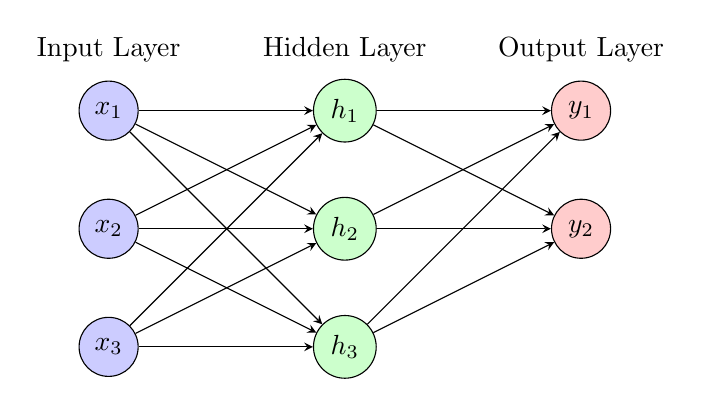
\begin{tikzpicture}[x=1.5cm, y=1.5cm, >=stealth]

            % Input Layer
            \foreach \i in {1,2,3}
            \node[circle, draw, fill=blue!20, minimum size=0.75cm] (I\i) at (0,-\i) {$x_{\i}$};

            % Hidden Layer
            \foreach \i in {1,2,3}
            \node[circle, draw, fill=green!20, minimum size=0.75cm] (H\i) at (2,-\i) {$h_{\i}$};

            % Output Layer
            \foreach \i in {1,2}
            \node[circle, draw, fill=red!20, minimum size=0.75cm] (O\i) at (4,-\i) {$y_{\i}$};

            % Connect Layers
            \foreach \i in {1,2,3}
            \foreach \j in {1,2,3}
            \draw[->] (I\i) -- (H\j);

            \foreach \i in {1,2,3}
            \foreach \j in {1,2}
            \draw[->] (H\i) -- (O\j);

            % Labels
            \node[above=0.5cm] at (I1) {Input Layer};
            \node[above=0.5cm] at (H1) {Hidden Layer};
            \node[above=0.5cm] at (O1) {Output Layer};

        \end{tikzpicture}
    \end{center}
    \caption{Neural Network con 1 hidden layer}
\end{figure}

\subsection{Gli ingredienti di una rete neurale}
\subsubsection{Il grafo g}
Un grafo $g = \{N,E\}$ è un grafo diretto pesato con label.

Ogni nodo $i \in N$ viene chiamato \textbf{neurone} o \textbf{percettrone}. Per
ogni nodo ci sono 2 targhette:
\begin{itemize}
    \item Un valore $a_i$ che viene chiamato \textbf{attivazione}
    \item Una funzione di attivazione $f_i$ che viene applicata all'attivazione, che
          produce un output $z_i$
\end{itemize}

Ogni arco $e = \{j \in N \rightarrow i \in N\} \in E$ associato con un peso
$w_{j,i}$.

Ogni nodo $i$ è anche coinvolto con un arco speciale, con un nodo fantasma, che
viene chiamato \textbf{bias} $b_i$.

\textbf{Nota:} $z_i = f_i(a_i)$. E $a_i = b_i  + \sum_{j:j\rightarrow i \in E} w_{j,i}z_j$

La combinazione dei neuroni connessi costruisce il grafo. I nodi che
condividono gli stessi input sono raggruppati in \textbf{layers}.

\usetikzlibrary{positioning}
\begin{figure}[H]
    \begin{center}

        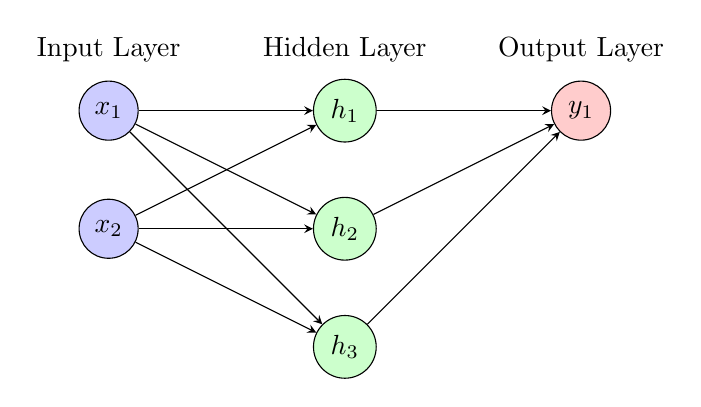
\begin{tikzpicture}[x=1.5cm, y=1.5cm, >=stealth]

            % Input Layer
            \foreach \i in {1,2}
            \node[circle, draw, fill=blue!20, minimum size=0.75cm] (I\i) at (0,-\i) {$x_{\i}$};

            % Hidden Layer
            \foreach \i in {1,2,3}
            \node[circle, draw, fill=green!20, minimum size=0.75cm] (H\i) at (2,-\i) {$h_{\i}$};

            % Output Layer
            \foreach \i in {1}
            \node[circle, draw, fill=red!20, minimum size=0.75cm] (O\i) at (4,-\i) {$y_{\i}$};

            % Connect Layers
            \foreach \i in {1,2}
            \foreach \j in {1,2,3}
            \draw[->] (I\i) -- (H\j);

            \foreach \i in {1,2,3}
            \foreach \j in {1}
            \draw[->] (H\i) -- (O\j);

            % Labels
            \node[above=0.5cm] at (I1) {Input Layer};
            \node[above=0.5cm] at (H1) {Hidden Layer};
            \node[above=0.5cm] at (O1) {Output Layer};

        \end{tikzpicture}
    \end{center}
    \caption{Neural Network con 1 hidden layer}
\end{figure}

Il risultato finale dipende da tutti i parametri del grafo, e anche dal tipo di
funzione di attivazione che viene usata.
\begin{quote}
    Ma come facciamo a scegliere il corretto valore dei parametri del grafo?
\end{quote}

\subsubsection{La funzione di loss}
Il grafo è un operatore algebrico non lineare: $g(\vec{x}|W,B)$. In questo
grafo non sappiamo il valore di \textbf{B e W}. La fase di apprendimenti di una
rete consiste nel trovare il \textbf{migliore} valore per W e per B. Ma cosa
intendiamo con \textbf{migliore?}.

Formalmente, l'unico modo che abbiamo per definire la conezione di migliore, è
quello di \textit{approssimare al meglio la funzione che vogliamo trovare}.

%scrivi un vettore verticale di x_1 a x_m e un vettore verticale di y_1 a y_m%

Consideriamo il valore di una funzione $F$ su $x_i$ e il vero valore di $y_i$.
Noi vogliamo minimizzare la differenza tra $F(x_i)$ e $y_i$.

\begin{equation}
    \min_{W,B}\frac{1}{n} \sum_{i=1}^n loss(\vec{y_i}, g(x_i|W,B))
\end{equation}
con:
\begin{itemize}
    \item $loss(\vec{y_i}, g(x_i|W,B))$ è una funzione che misura la differenza tra $y_i$ e $g(x_i|W,B)$
    \item $n$ è il numero di esempi
    \item $W$ e $B$ sono i parametri del grafo
    \item $g(x_i|W,B)$ è il valore di output del grafo
    \item $\vec{y_i}$ è il valore di output vero
\end{itemize}

La funzione di \textbf{loss} dipende dal tipo di task che dobbiamo svolgere.

\subsubsection{Funzione di loss per Regressione}
\textbf{Mean Absolute Error}:
\begin{equation}
    \frac{1}{n} \sum_{i=1}^n |y_i - g(\vec{x_i}|W,B)|
\end{equation}
\begin{itemize}
    \item Considera tutti gli errori con lo stesso peso
    \item \textbf{Non è differenziabile in 0}
\end{itemize}

\textbf{Mean Squared Error}:
\begin{equation}
    \frac{1}{n} \sum_{i=1}^n (y_i - g(\vec{x_i}|W,B))^2
\end{equation}

\begin{itemize}
    \item Gli errori più grandi hanno un peso maggiore
    \item \textbf{È differenziabile in 0}
    \item \textbf{È più sensibile agli outliers}
\end{itemize}

\textbf{Domanda:} quale si usa tra le due? Dall'approccio greedy, \textbf{usa entrambe}.

\textbf{Esistono anche altre funzioni:}
\begin{itemize}
    \item Smooth Absolute Error
    \item Huber Loss
\end{itemize}

\subsubsection{Funzione di loss per classificazione}

\textbf{Binary Cross Entropy [BCE]}
Viene usata se $y_i \in \{0,1\}, g(\vec{x}|W,B) \in [0,1]$.
\begin{equation}
    BCE = -\frac{1}{n} \sum_{i=1}^n y_i \log(g(\vec{x_i}|W,B)) - (1-y_i)\log(1-g(\vec{x_i}|W,B))
\end{equation}

\textbf{Categorical Cross Entropy [CCE]}
Da scrivere.

\subsection{L'ottimizzatore o}
Come risolviamo il problema di:
\begin{equation}
    \min_{W,B} \frac{1}{n} \sum_{i=1}^n loss(\vec{y_i}, g(\vec{x_i}|W,B))
\end{equation}

Il problema lo risolviamo calcolando il \textbf{gradiante} della funzione loss,
lo poniamo uugale a 0 e controlliamo se siamo in un punto di \textbf{massimo,
    minimo o punto di sella}.

\begin{tikzpicture}
    \begin{axis}[
            xlabel=$x$,
            ylabel=$f(x)$,
            domain=-2:2,
            samples=200,
            axis lines=middle,
            width=10cm,
            height=6cm,
            xmin=-2,
            xmax=2,
            ymin=-4,
            ymax=5,
            xtick={-1, 0, 1},
            xticklabels={$-1$, $0$, $1$},
            ytick={1, 3},
            yticklabels={$f_{\text{min}}$, $f_{\text{max}}$},
        ]

        \addplot[blue,thick,domain=-1.5:1.5] {x^4 - 2*x^3 - 2*x^2 + 3*x + 1};
    \end{axis}
\end{tikzpicture}

Abbiamo bisogno di un metodo iterativo per trovare una soluzione. Ci vuole
un'\textbf{euristica}. Tipicamente, siamo soddisfatti di un \textbf{minimo
    locale}, e si utilizza, appunto, il \textbf{metodo di discesa del gradiente}.

\subsubsection{Il metodo di discesa del gradiente}
Sia $F(\vec{x})$ una funzione differenziabile.
\begin{itemize}
    \item $F(\vec{x})$ decresce più veloce nella direzione del gradiente negativo
    \item $F(\vec{x})$ cresce più veloce nella direzione opposta al gradiente
\end{itemize}

\begin{equation}
    a^{new} = a^{old} - \eta \cdot \nabla F(a^{old})
\end{equation}

Il parametro $\eta$ viene chiamato \textbf{learning rate} e determina il
comportamento del'ottimizzazione.
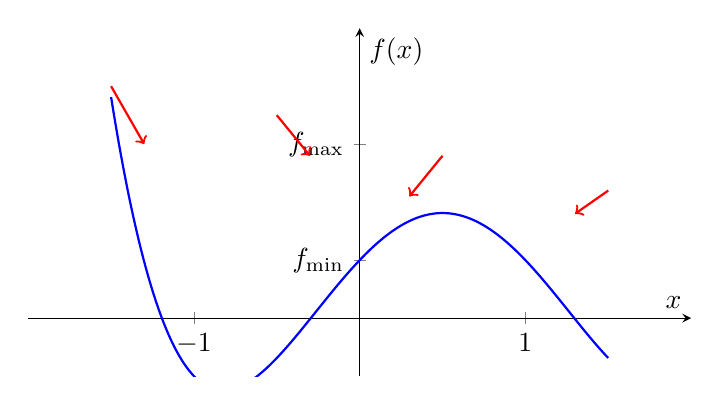
\begin{tikzpicture}
    \begin{axis}[
            xlabel=$x$,
            ylabel=$f(x)$,
            domain=-2:2,
            samples=200,
            axis lines=middle,
            width=10cm,
            height=6cm,
            xmin=-2,
            xmax=2,
            ymin=-1,
            ymax=5,
            xtick={-1, 0, 1},
            xticklabels={$-1$, $0$, $1$},
            ytick={1, 3},
            yticklabels={$f_{\text{min}}$, $f_{\text{max}}$},
        ]

        \addplot[blue,thick,domain=-1.5:1.5] {x^4 - 2*x^3 - 2*x^2 + 3*x + 1};

        % Frecce verso il minimo
        \draw[->, red, thick] (axis cs:-1.5,4) -- (axis cs:-1.3,3);
        \draw[->, red, thick] (axis cs:-0.5,3.5) -- (axis cs:-0.3,2.8);
        \draw[->, red, thick] (axis cs:0.5,2.8) -- (axis cs:0.3,2.1);
        \draw[->, red, thick] (axis cs:1.5,2.2) -- (axis cs:1.3,1.8);

    \end{axis}
\end{tikzpicture}

\textbf{Ci sono ancora problemi:} Questo metodo non è esente da problemi, quindi abbiamo:
\begin{itemize}
    \item Dipendentemente dal punto di inizio, abbiamo un risultato diverso. Dobbiamo
          capire che, giustamente, se ci accontentiamo di un minimo locale, non avremo
          quasi mai lo stesso minimo per ogni allenamento della rete.
\end{itemize}

Diciamo che in generale, gli steps per allenare una rete sono:
\lstset{mathescape}
\begin{lstlisting}
    for each topology T in $C_t$
        for each $\eta$ in $C_\eta$
            for each initialization I in $C_I$
                Applica la discesa del gradiente
\end{lstlisting}

\subsubsection{Il metodo di discesa del gradiente stocastico}
La differenza del metodo di discesa del gradiente stocastico è che, invece di
calcolare il gradiente su tutti i dati, si calcola il gradiente su un
sottoinsieme di dati.

Ciò che viene fatto, per ogni step, invece di prendere la derivata di ogni loss
function e poi fare i calcoli, prendo \textbf{un sample del mio dataset},
tipicamente chiamato \textbf{batch}. Ogni volta che calcolo la discesa del
gradiente, calcolo la derivata \textbf{NON PER TUTTO IL DATASET}, ma solamente
del \textbf{batch}. Questo OVVIAMENTE non mi assicura che ottimizzare ogni
batch mi ottimizza anche l'intero dataset, ma non c'è modo di lavorare
sull'intero dasaset, poiché questo è troppo grande e richiede troppo tempo.

Nonostante tutto, utilizzando questa tecnica \textbf{si ottengono risultati
    comunque accettabili}.

Il \textit{workflow} allora cambia in: \lstset{mathescape}
\begin{lstlisting}
    for each topology T in $C_t$
        for each $\eta$ in $C_\eta$
          for each initialization I in $C_I$
           for each batch size $b \in C_b$
             Applica la discesa del gradiente stocastica
\end{lstlisting}

\subsubsection{Linee guida sul learning rate}

\textbf{Epoca}: Un'epoca è un passaggio dell'approssimazione della funzione

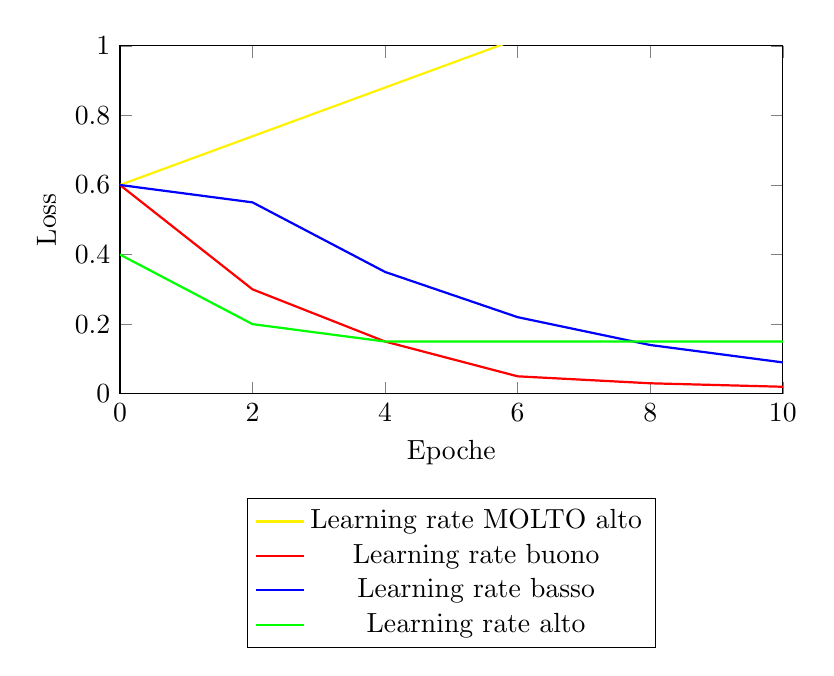
\begin{tikzpicture}
    \begin{axis}[
            xlabel=Epoche,
            ylabel=Loss,
            width=10cm,
            height=6cm,
            xmin=0,
            xmax=10,
            ymin=0,
            ymax=1,
            xtick={0, 2, 4, 6, 8, 10},
            ytick={0, 0.2, 0.4, 0.6, 0.8, 1},
            legend style={at={(0.5,-0.3)},anchor=north},
            legend entries={Learning rate MOLTO alto, Learning rate buono, Learning rate basso, Learning rate alto},
        ]

        \addplot[thick, yellow] coordinates {(0, 0.6) (10, 1.3)};
        \addplot[thick, red] coordinates {(0, 0.6) (2, 0.3) (4, 0.15) (6, 0.05) (8, 0.03) (10, 0.02)};
        \addplot[thick, blue] coordinates {(0, 0.6) (2, 0.55) (4, 0.35) (6, 0.22) (8, 0.14) (10, 0.09)};
        \addplot[thick, green] coordinates {(0, 0.4) (2, 0.2) (4, 0.15) (6, 0.15) (8, 0.15) (10, 0.15)};

    \end{axis}
\end{tikzpicture}

\textbf{Nota:} Il learning rate è un parametro che va \textbf{tunato}.
\begin{itemize}
    \item Se il learning rate è troppo alto, non si riesce a convergere poiché si
          salta il minimo
    \item Se il learning rate è troppo basso, si rischia di non convergere mai
\end{itemize}

Il nostro obiettivo è quello di avere un learning rate che sia \textbf{giusto} e che permetta di avere un andamento della funzione di loss come quello in rosso, cioé avere una buona
diminuizione della loss andando avanti con le epoche. Sempre decrescente e con la distanza minore dall'asse delle x.

\textbf{Domanda:} Vogliamo sempre la loss uguale a 0? \textbf{No.}
Perché? Perché a differenza che in statistica dove vogliamo avere un errore il minimo.
In deep learning non è così. Se la loss è 0, allora vuol dire che la rete ha
imparato a memoria i dati, e non è quello che vogliamo. Vogliamo che la rete
sia capace di generalizzare.

In particolare, noi \textbf{vogliamo fare predizioni}, sopratutto su \textbf{istanze ancora non viste.} Se avessimo una loss uguale a 0, probabilmente non 
saremmo in grado di avere delle predizioni decenti, poiché la rete non è in grado di generalizzare.
Avendo la loss non a 0 rendiamo la rete capace di poter introdurre istanze ancora non viste in futuro.

Quindi, per statistica \textbf{loss = 0 : nice}, per \textbf{deep learning: insomma}.


\begin{tikzpicture}
    \begin{axis}[
        xlabel=$x$,
        ylabel=$y$,
        width=12cm, % Larghezza maggiore
        height=6cm,
        xmin=0,
        xmax=10,
        ymin=0,
        ymax=1,
        xtick={0, 2, 4, 6, 8, 10},
        ytick={0, 0.2, 0.4, 0.6, 0.8, 1},
    ]
    
    \addplot[thick, blue, smooth] coordinates {(0, 1) (2, 0.5) (4, 0.3) (8, 0)};
    \end{axis}
    \end{tikzpicture}
\newpage
\section{Classificazione Binaria}
\textbf{Descrizione di cosa andremo a fare:} utilizziamo il dataset IMDb Dataset.
Questo dataset è un Database compilato dagli utenti del sito. Le caratteristiche, in particolare, sono:
\begin{itemize}
    \item 50.000 recensioni
    \item circa 50\% positive e 50\% negative
    \item \textit{25.000} sono usate per il \textbf{training} e \textit{25.000} sono usate per il \textbf{testing}. Anche queste sono il 50\% positive e 50\% negative.
\end{itemize}

La task che faremo su questo dataset prende il nome di \textbf{sentimental
    analysis}, ovvero analisi del sentimento.

\textbf{Assunzione:} Ciò che stiamo facendo ha senso solamente se assumiamo \textit{che nel futuro avremo punti con una distribuzione abbastanza simile a quelli utilizzati per il training}.

La partizione di \textbf{test} è una partizione che non viene utilizzata per la
fase di training, ma viene utilizzata successivamente per controllare se il
modello si sta comportando bene nella predizione dei valori. Ci sono delle
misure che hanno range $[0,1]$ che ci permettono di capire quanto il modello si
sta comportando bene.

\textbf{Nota:} il \textit{test set} non viene fornito quando si lavora nel deep learning, altrimenti verrebbe usato per ottimizzare direttamente il modello. \textbf{Non si conosce inizialmente.}

% BEGIN: xz8c6549bwf9
\begin{figure}[H]
    \centering
    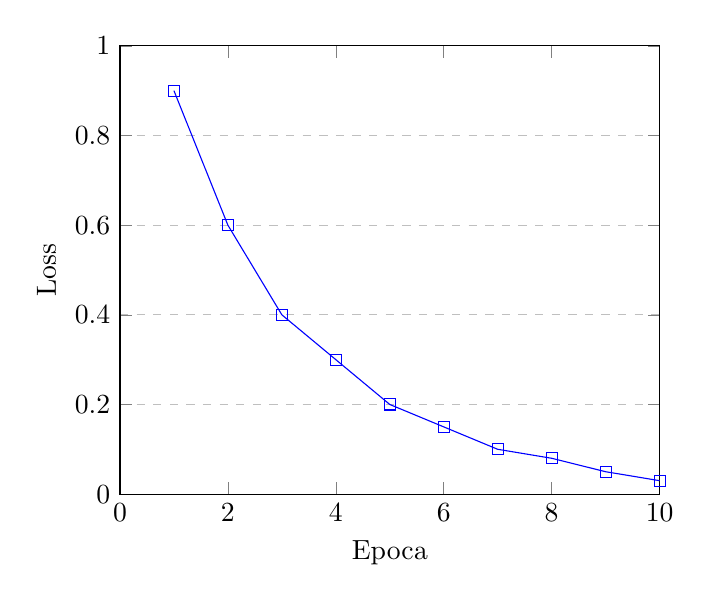
\begin{tikzpicture}
        \begin{axis}[
                xlabel={Epoca},
                ylabel={Loss},
                xmin=0, xmax=10,
                ymin=0, ymax=1,
                xtick={0,2,4,6,8,10},
                ytick={0,0.2,0.4,0.6,0.8,1},
                legend pos=north east,
                ymajorgrids=true,
                grid style=dashed,
            ]
            \addplot[
                color=blue,
                mark=square,
            ]
            coordinates {
                    (1,0.9)(2,0.6)(3,0.4)(4,0.3)(5,0.2)(6,0.15)(7,0.1)(8,0.08)(9,0.05)(10,0.03)
                };
        \end{axis}
    \end{tikzpicture}
    \caption{Grafico di una curva di loss che diminuisce all'aumentare delle epoche.}
    \label{fig:loss_curve}
\end{figure}
% END: xz8c6549bwf9

\subsection{Caricamento e gestione del Dataset}

\begin{lstlisting}[language=Python, caption=Caricamento del dataset IMDb Dataset.]
from keras.datasets import imdb
(train_data, train_labels), (test_data, test_labels) = imdb.load_data(num_words=10000)
\end{lstlisting}

\begin{itemize}
    \item training\_data: sono gli input del training
    \item training\_labels: sono gli output del training
    \item test\_data: sono gli input del test
    \item test\_labels: sono gli output del test
\end{itemize}

% BEGIN: 7z5t8f6d4xw3
\begin{figure}[H]
    \centering
    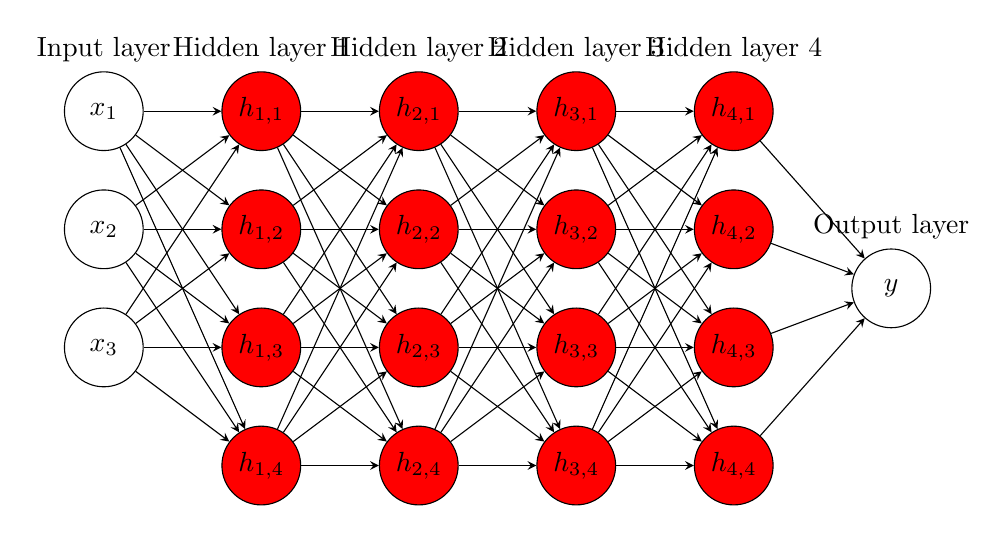
\begin{tikzpicture}[x=1cm, y=1.5cm, >=stealth]
        % Input layer nodes
        \foreach \i in {1,...,3}
        \node[circle, draw=black, fill=white, inner sep=0pt, minimum size=10mm] (I-\i) at (0,-\i) {$x_\i$};

        % Hidden layer nodes
        \foreach \i in {1,...,4}
        \node[circle, draw=black, fill=red, inner sep=0pt, minimum size=10mm] (H1-\i) at (2,-\i) {$h_{1,\i}$};
        \foreach \i in {1,...,4}
        \node[circle, draw=black, fill=red, inner sep=0pt, minimum size=10mm] (H2-\i) at (4,-\i) {$h_{2,\i}$};
        \foreach \i in {1,...,4}
        \node[circle, draw=black, fill=red, inner sep=0pt, minimum size=10mm] (H3-\i) at (6,-\i) {$h_{3,\i}$};
        \foreach \i in {1,...,4}
        \node[circle, draw=black, fill=red, inner sep=0pt, minimum size=10mm] (H4-\i) at (8,-\i) {$h_{4,\i}$};

        % Output layer nodes
        \node[circle, draw=black, fill=white, inner sep=0pt, minimum size=10mm] (O) at (10,-2.5) {$y$};

        % Connections
        \foreach \source in {1,...,3}
        \foreach \dest in {1,...,4}
        \draw[->] (I-\source) -- (H1-\dest);
        \foreach \source in {1,...,4}
        \foreach \dest in {1,...,4}
        \draw[->] (H1-\source) -- (H2-\dest);
        \foreach \source in {1,...,4}
        \foreach \dest in {1,...,4}
        \draw[->] (H2-\source) -- (H3-\dest);
        \foreach \source in {1,...,4}
        \foreach \dest in {1,...,4}
        \draw[->] (H3-\source) -- (H4-\dest);
        \foreach \source in {1,...,4}
        \draw[->] (H4-\source) -- (O);

        % Labels
        \node[above] at (I-1.north) {Input layer};
        \node[above] at (H1-1.north) {Hidden layer 1};
        \node[above] at (H2-1.north) {Hidden layer 2};
        \node[above] at (H3-1.north) {Hidden layer 3};
        \node[above] at (H4-1.north) {Hidden layer 4};
        \node[above] at (O.north) {Output layer};
    \end{tikzpicture}
    \caption{Neural network with 3 input nodes, 4 hidden layers with 3 nodes each, and 1 output layer with 1 node.}
    \label{fig:neural_network}
\end{figure}

Quali sono i primi problemi che vanno gestiti in questo caso? Abbiamo il
problema che i \textbf{dati sono parole e non numeri}. Quindi dobbiamo
trasformare le parole in numeri.

Ogni parola viene \textbf{trasformato} in un numero. Ci troviamo però con delle
recensioni che sono delle \textbf{sequenze di parole}, e quindi abbiamo delle
\textbf{sequenze di numeri}. La soluzione è quelal di usare un \textbf{set di
    parole codificate.} Mi spiego:

Immaginiamo di avere 10.000 parole encodate. Salvo queste 10.000 parole in un
array e associo ad ogni parola un indice di questo array.

\begin{figure}[H]
    \begin{center}
        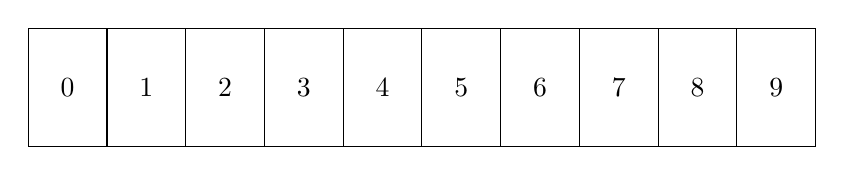
\begin{tikzpicture}[x=1cm, y=1.5cm, >=stealth]
            \draw (0,0) rectangle (10,1);
            \draw (0,0) rectangle (1,1);
            \draw (1,0) rectangle (2,1);
            \draw (2,0) rectangle (3,1);
            \draw (3,0) rectangle (4,1);
            \draw (4,0) rectangle (5,1);
            \draw (5,0) rectangle (6,1);
            \draw (6,0) rectangle (7,1);
            \draw (7,0) rectangle (8,1);
            \draw (8,0) rectangle (9,1);
            \draw (9,0) rectangle (10,1);
            \node at (0.5,0.5) {0};
            \node at (1.5,0.5) {1};
            \node at (2.5,0.5) {2};
            \node at (3.5,0.5) {3};
            \node at (4.5,0.5) {4};
            \node at (5.5,0.5) {5};
            \node at (6.5,0.5) {6};
            \node at (7.5,0.5) {7};
            \node at (8.5,0.5) {8};
            \node at (9.5,0.5) {9};
        \end{tikzpicture}

    \end{center}
\end{figure}

Ora, cosa manca? \textbf{Manca l'ordine}. L'unica cosa che abbiamo è quindi una
indicizzazione delle parole, ma non abbiamo alcuna informazione dell'ordine.
\textbf{Manca anche totalmente la semantica}.

La struttura dell'input è quindi un \textbf{livello con 10.000 nodi di input.s}

\textbf{Input}
\begin{lstlisting}[language=Python]
import numpy as np
def vectorize_sequences(sequences, dimension=10000):
# Create an all-zero matrix of shape (len(sequences), dimension)
results = np.zeros((len(sequences), dimension))
for i, sequence in enumerate(sequences):
    results[i, sequence] = 1. # set specific indices of results[i] to 1s
return results
# Our vectorized training data
x_train = vectorize_sequences(train_data)
# Our vectorized test data
x_test = vectorize_sequences(test_data)

\end{lstlisting}

\textbf{Output}
\begin{lstlisting}[language=Python]
# Our vectorized labels
y_train = np.asarray(train_labels).astype('float32')
y_test = np.asarray(test_labels).astype('float32')

\end{lstlisting}

\subsection{Definizione della Rete Neurale}
\textbf{Codice iniziale della definizione della Rete}

\begin{lstlisting}[language=Python]
    from keras import models
from keras import layers
model = models.Sequential()
model.add(layers.Dense(16, activation='relu', input_shape=(10000,)))
model.add(layers.Dense(16, activation='relu'))
model.add(layers.Dense(1, activation='sigmoid'))
model.compile(optimizer='rmsprop', 
            loss='binary_crossentropy',
             metrics=['accuracy'])
\end{lstlisting}

Il \textbf{modello sequenziale} è quello migliore da dove iniziare. Cosa
significa però modello sequenziale? Il modello sequenziale ha il concetto di
\textbf{layer}. Ha la funzione \textbf{add} che aggiunge un layer sopra gli
altri layer che sono già esistenti.

\textbf{Primo Layer:}

\textit{layers.Dense}: un layer denso significa che ogni nodo di quel layer è collegato con ogni nodo del layer precedente. \textbf{16} è il numero di neuroni che si vogliono attivare in quel layer.
input\_shape è la dimensione dell'input. \textbf{10000} è la dimensione dell'input. Notare che si ha una \textbf{virgola} nell'input dopo il 10.000 e indica che \textit{che stiamo aspettando una sequenza di vettori, ognuno di dimensione 10.000}
Cioè, praticamente stiamo dicendo \textbf{10.000} sono le parole per ogni recensione, e con la virgola stiamo dicendo che \textbf{non sappiamo quante recensioni abbiamo}.E' comodo quando non abbiamo un numero
fisso di example del dataset da processare.

\textbf{Quante connessioni ci sono?} \[16 \cdot 10000 + 16 = 160016\] dove sono 16 i bias.

\textbf{Cosa significa relu?} ReLu è la funzione di attivazione.

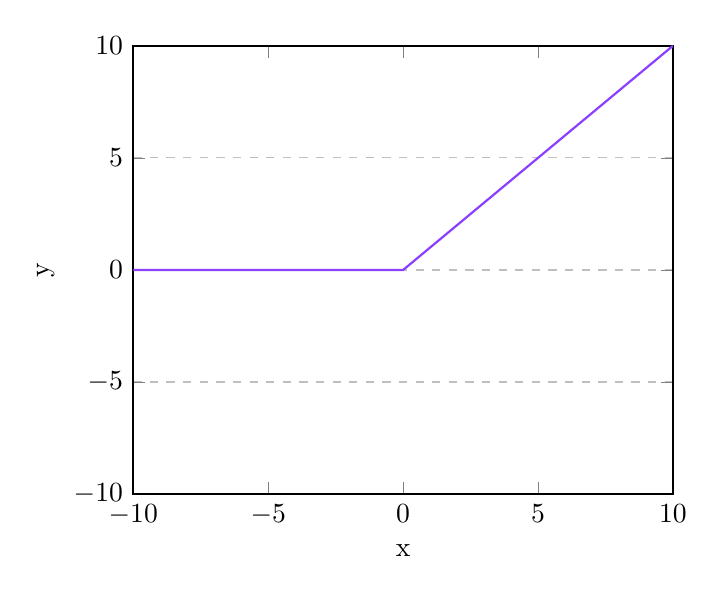
\begin{tikzpicture}
    \begin{axis}[
            xlabel={x},
            ylabel={y},
            xmin=-10, xmax=10,
            ymin=-10, ymax=10,
            xtick={-10,-5,0,5,10},
            ytick={-10,-5,0,5,10},
            legend pos=north east,
            ymajorgrids=true,
            grid style=dashed,
            thick
        ]
        \addplot[
            color=custompurple,
            thick
        ]
        coordinates {
                (-10,0)(-9,0)(-8,0)(-7,0)(-6,0)(-5,0)(-4,0)(-3,0)(-2,0)(-1,0)(0,0)(1,1)(2,2)(3,3)(4,4)(5,5)(6,6)(7,7)(8,8)(9,9)(10,10)
            };
    \end{axis}
\end{tikzpicture}

E' una funzione di attivazione artificiale che fino a 0 è 0, e poi cresce
linearmente. E' una funzione che si usa molto in deep learning.

\textbf{Secondo layer}:

Nel secondo layer abbiamo altri \textbf{16} nodi connessi con i precedenti 16
nodi. In tutto abbiamo \[16 \cdot 16 + 16 = 272\] connessioni, con 16 che sono i bias.

\textbf{Layer di output}:

In questo layer abbiamo un unico nodo connesso con i 16 nodi precedenti. In
tutto abbiamo \[16 \cdot 1 + 1 = 17\] connessioni, con 1 che è il bias. La funzione di attivazioe è la
\textbf{sigmoid}, che è una funzione che ha range $[0,1]$ che indica la
probabilità che il dato appartenga alla classe 1.

Diciamo che è stato osservato che la \textit{sigmoid è meglio nell'output}.
Perché? Eh funziona cosi a quanto pare lol.

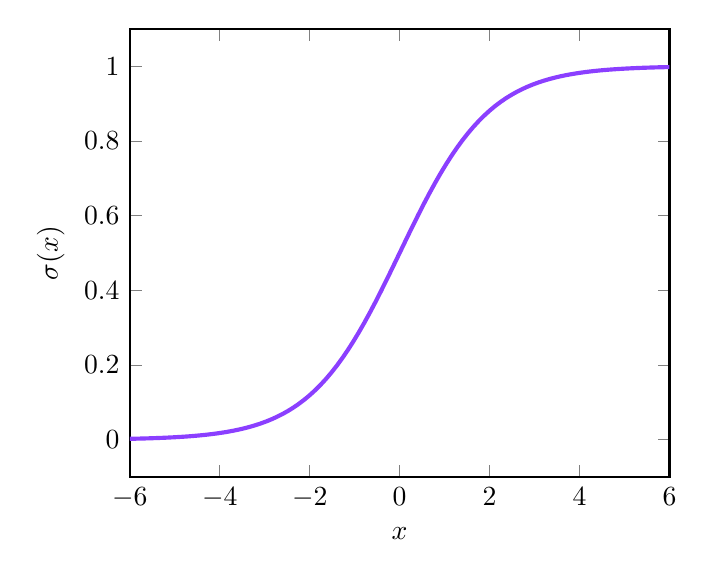
\begin{tikzpicture}
    \begin{axis}[
            xlabel=$x$,
            ylabel=$\sigma(x)$,
            xmin=-6, xmax=6,
            ymin=-0.1, ymax=1.1,
            samples=100,
            thick,
            every axis plot/.append style={line width=1.5pt}
        ]
        \addplot[custompurple,domain=-6:6] {1/(1+exp(-x))};
    \end{axis}
\end{tikzpicture}

\textbf{Compilazione del modello}

In questa sezione si definisce il \textbf{loss} e l'\textbf{optimizer}.

L'ottimizzatore sarebbe, praticamente, la \textit{discesa del gradiente}. Ci
sono vari ottimizzatori ed è molto buono per te stesso provare gli
ottimizzatori e vedere quale funziona meglio per il tuo problema. Letteralmente
il deep learning :) Per quanto riguarda la loss abbiamo visto nella scorsa
sezione le funzioni di loss che conosciamo.

La \textbf{metrica} è quella che viene usata per valutare effettivamente il
modello. In questo caso si usa l'\textbf{accuracy} che praticamente è la
percentuale di classificazioni corrette.

\subsection{Plotting del modello}

E' un plotting molto base e non molto fancy, ma fa il suo lavoro diciamo
\begin{lstlisting}[language=Python]
from keras.utils import plot_model
plot_model(model, show_shapes=True, show_layer_names=True)
    
\end{lstlisting}

\begin{figure}[H]
    \centering
    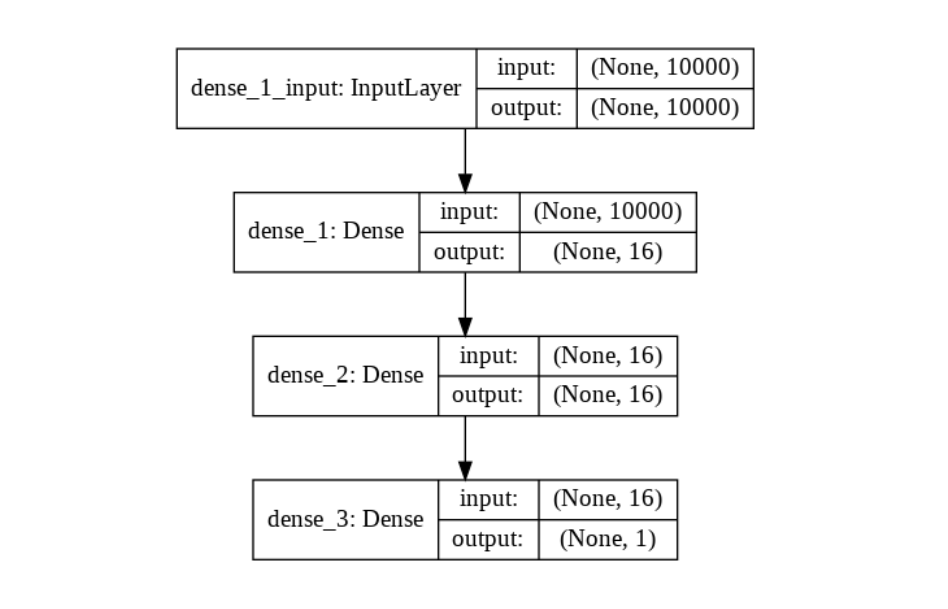
\includegraphics[width=0.8\linewidth]{images/plot res.png}
    \caption{Plotting del modello.}
    \label{fig:plot_model}
\end{figure}

\subsection{Training del modello e valutazione}

Entra in gioco il concetto di \textbf{validation set}.

\subsubsection{Validation Set}
Quando ho un modello, come faccio a sapere se la rete che sto allenando si sta
allenando in modo corretto? Tutto questo sapendo che \textbf{non abbiamo
    accesso al test set}. Pensiamo al \textbf{training set} e pensiamo ad un altro
\textbf{split} interno al training set:
\begin{itemize}
    \item Training set parziale
    \item Validation set
\end{itemize}

Quindi se avessimo 50.000 di grandezza del dataset:
\begin{itemize}
    \item 25.000 test set
    \item 25.training set
          \begin{itemize}
              \item 10.000 validation set
              \item 15.000 training set parziale
          \end{itemize}
\end{itemize}

\begin{lstlisting}
x_val = x_train[:10000]
partial_x_train = x_train[10000:]
y_val = y_train[:10000]
partial_y_train = y_train[10000:]

\end{lstlisting}

Praticamente è come se usassimo il validation come se fosse un test set. Quindi
andremo a plottare 2 curve:
\begin{itemize}
    \item La loss sulle epoche
    \item L'accuracy sulle epoche
\end{itemize}

\textbf{La loss} ci da un'idea di quanto il modello si sta allenando bene. Se ci sono problemi, la figura è strana e non segue un andamento corretto, si modifica.
Ma la cosa importante è la \textbf{validation accuracy}, che DEVE essere crescere in modo monotono e deve avvicinarsi a 1 il più possibile.

%grafico loss
\begin{figure}[H]
    \centering
    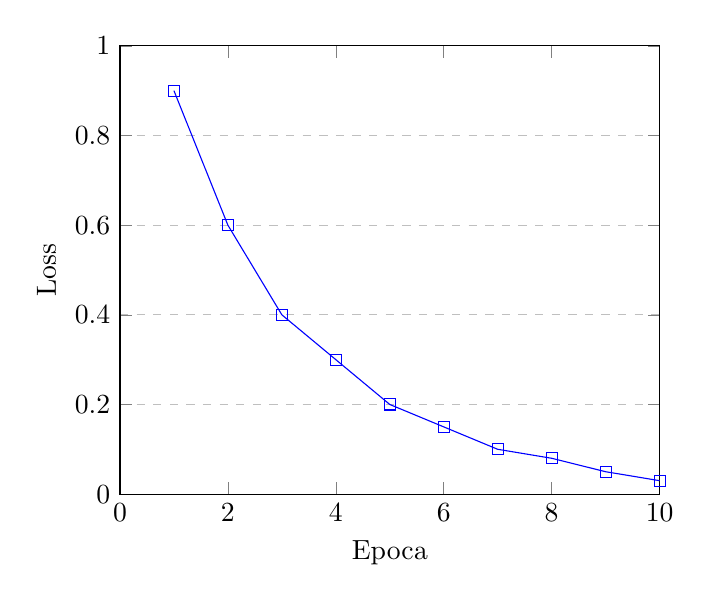
\begin{tikzpicture}
        \begin{axis}[
                xlabel={Epoca},
                ylabel={Loss},
                xmin=0, xmax=10,
                ymin=0, ymax=1,
                xtick={0,2,4,6,8,10},
                ytick={0,0.2,0.4,0.6,0.8,1},
                legend pos=north east,
                ymajorgrids=true,
                grid style=dashed,
            ]
            \addplot[
                color=blue,
                mark=square,
            ]
            coordinates {
                    (1,0.9)(2,0.6)(3,0.4)(4,0.3)(5,0.2)(6,0.15)(7,0.1)(8,0.08)(9,0.05)(10,0.03)
                };
        \end{axis}
    \end{tikzpicture}
    \caption{Grafico di una curva di loss che diminuisce all'aumentare delle epoche.}
    \label{fig:loss_curve}
\end{figure}

%grafico accuracy
\begin{figure}[H]
    \centering
    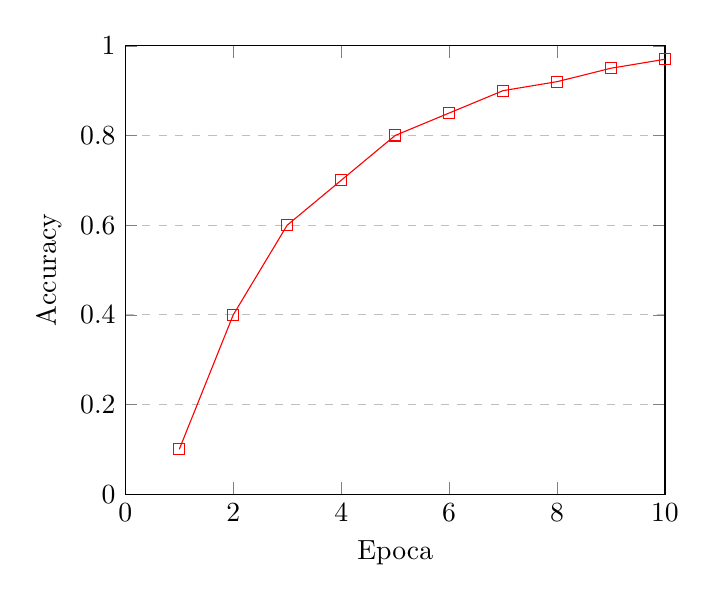
\begin{tikzpicture}
        \begin{axis}[
                xlabel={Epoca},
                ylabel={Accuracy},
                xmin=0, xmax=10,
                ymin=0, ymax=1,
                xtick={0,2,4,6,8,10},
                ytick={0,0.2,0.4,0.6,0.8,1},
                legend pos=north east,
                ymajorgrids=true,
                grid style=dashed,
            ]
            \addplot[
                color=red,
                mark=square,
            ]
            coordinates {
                    (1,0.1)(2,0.4)(3,0.6)(4,0.7)(5,0.8)(6,0.85)(7,0.9)(8,0.92)(9,0.95)(10,0.97)
                };
        \end{axis}
    \end{tikzpicture}
    \caption{Grafico di una curva di accuracy che aumenta all'aumentare delle epoche.}
    \label{fig:accuracy_curve}
\end{figure}

Ma anche se avessimo queste curve inìcon questa conformazione, \textbf{ancora
    non ci dice niente}. Il validation è in un senso insensato per l'output. Ciò
che importerà sarà il \textbf{test set} che non è stato usato per il training.

\textbf{Training code}

\begin{lstlisting}[language=Python]
history = model.fit(partial_x_train,
            partial_y_train,
            epochs=20,
            batch_size=512,
            validation_data=(x_val, y_val))
\end{lstlisting}

\textbf{Plotting delle curve}

Notare che questo è un plotting molto base e non molto fancy, e in futuro
utilizzeremo \textbf{Tensorboard} che aggiornerà in tempo reale i grafici

\begin{lstlisting}[language=Python]
import matplotlib.pyplot as plt
loss = history.history['loss']
val_loss = history.history['val_loss']
epochs = range(1, len(loss) + 1)
# "bo" is for "blue dot"
plt.plot(epochs, loss, 'bo', label='Training loss')
# b is for "solid blue line"
plt.plot(epochs, val_loss, 'b', label='Validation loss')
plt.title('Training and validation loss')
plt.xlabel('Epochs')
plt.ylabel('Loss')
plt.legend()
plt.show()
\end{lstlisting}

Notare che \textit{history} è un dizionario e si può accedere come indicato a
riga \textit{1 e 2} come accedere a loss e val\_loss.
\begin{figure}[H]
    \centering
    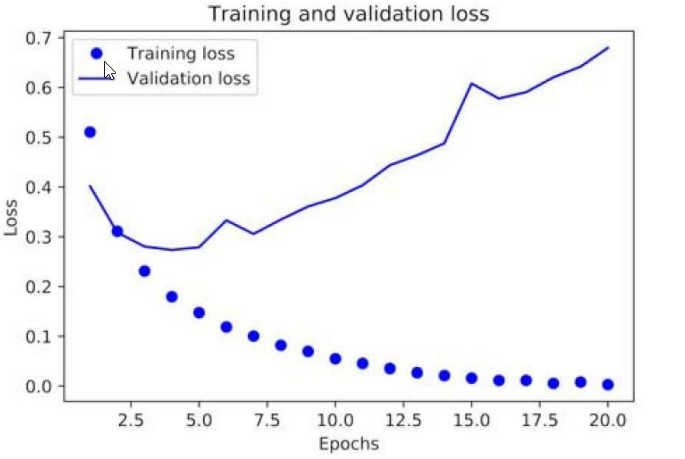
\includegraphics[width=0.8\linewidth]{images/wrong network.png}
    \caption{Rete sbagliata}
    \label{fig:loss}
\end{figure}

Un grafico del genere ci mostra una rete che \textbf{funziona male}!.

\begin{lstlisting}[language=Python]
plt.clf() # clear figure
acc = history_dict['binary_accuracy']
val_acc = history_dict['val_binary_accuracy']
plt.plot(epochs, acc, 'bo', label='Training acc')
plt.plot(epochs, val_acc, 'b', label='Validation acc')
plt.title('Training and validation accuracy')
plt.xlabel('Epochs')
plt.ylabel('Accuracy')
plt.legend()
plt.show()

\end{lstlisting}

\begin{figure}[H]
    \centering
    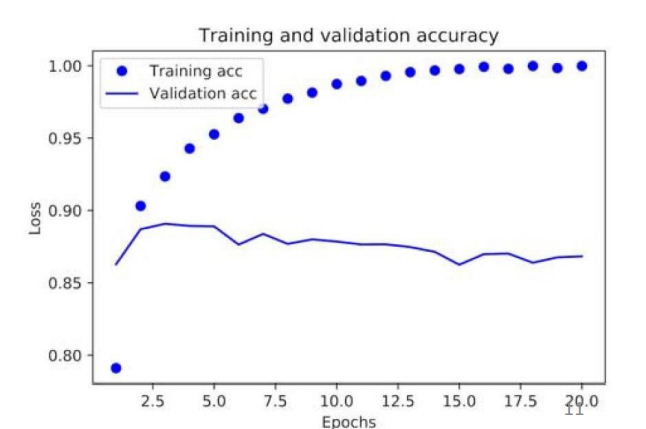
\includegraphics[width=0.8\linewidth]{images/overfitting.png}
    \caption{Overfitting}
    \label{fig:overfitting}
\end{figure}

In questo caso la rete ha un problema di \textbf{overfitting!}.

\subsection{Prediction}
\begin{lstlisting}
model.predict(x_test)
\end{lstlisting}
\[array([[ 0.91966152], [ 0.86563045], [ 0.99936908], ..., [ 0.45731062], [
                    0.0038014 ], [ 0.79525089]], dtype=float32\]

\subsection{Come risolvere problemi di accuracy bassa?}
Se quando andiamo a fare la validazione della nostra rete, come sappiamo come
modificare qualcosa per rendere la rete migliore? Ci sono alcuni approcci per
farlo:
\begin{itemize}
    \item Cambiare la topologia
    \item Diminuire le epoche
    \item Cambiare il numero di nodi per qualche layer
    \item FORSE cambiare anche il learning rate
\end{itemize}

Si noti che facendo questo vanno interpretati i grafici per capire come sta
andando la rete. Quando cominciamo a vedere che la \textbf{validation accuracy}
\textbf{NON STA SOLAMENTE CRESCENDO} ma ci sono dei punti in cui diminuisce,
siamo sicuri che \textbf{c'è qualche problema di mezzo.} Bisogna capire anche
su cosa lavorare. Se cambiando i dati spesso la \textbf{validation accuracy}
mostra problemi, allora bisogna lavorare per quello e cercare di trovare un
modo per fare in modo che il problema non si presenti.

\textbf{RECAPPONE}: Se notiamo che nella LOSS ci sono problemi, possiamo tunare il \textbf{learning rate} e altri
parametri per cercare di risolvere questi problemi. Ma la cosa più importante è \textbf{la metrica}. Se notiamo che
la \textbf{metrica non rispecchia un andamento di effettivo apprendimento}, capiamo che la rete non si sta comportando nel modo corretto
e non sta funzionando.

\subsection{Early Stopping}

E' un metodo che consiste nel vedere quando \textbf{la loss} comincia ad avere
dei comportamenti sospetti. Quando si \textbf{ferma} la rete in un dato
momento, si impedisce alla rete di \textbf{overfittare} nella maggior parte dei
casi.

\section{Classificazione Multiclasse}

Questa sezione sarà molto corta, poiché praticamente è la stessa cosa della
classificazione binaria, ma il layer finale della rete non sarà composto da un
solo nodo, ma da \textbf{un numero di nodi pari al numero di classi da
    classificare}.

\subsection{Descrizione del dataset - Reuters}

Il dataset che verrà utilizzato è il \textbf{Reuters Dataset}, che è un dataset
di \textbf{news} che sono state classificate in \textbf{46 categorie}. Ogni
categoria ha almeno 10 esempi nel training set.

\textbf{Preprocessing dell'input}

\begin{lstlisting}[language=Python]
import numpy as np
def vectorize_sequences(sequences, dimension=10000):
    results = np.zeros((len(sequences), dimension))
    for i, sequence in enumerate(sequences):
        results[i, sequence] = 1.
    return results
# Our vectorized training data
x_train = vectorize_sequences(train_data)
# Our vectorized test data
x_test = vectorize_sequences(test_data)
\end{lstlisting}

\subsubsection{Come processiamo l'output?}

Nel deep learning, \textbf{gli output categorici} non vengono mai mappati ad
una scala numerica. Si utilizza una tecnica che si chiama \textbf{one hot
    encoding}.

\textbf{One Hot Encoding}:

Consiste nel creare tante variabili numeriche quanti sono i valori della
variabile categorica, e per quel dato example viene assegnato
\begin{itemize}
    \item 1: se il valore della variabile categorica è quello
    \item 0: se il valore della variabile categorica non è quello, quindi in tutti gli altri casi
\end{itemize}

Da notare che il one hot encoding viene fatto sia per le labels di output, ma
non è sbagliato farlo anche per gli attributi in alcuni casi.

\begin{lstlisting}[language=Python]
def to_one_hot(labels, dimension=46):
    results = np.zeros((len(labels), dimension))
    for i, label in enumerate(labels):
        results[i, label] = 1.
    return results
# Our vectorized training labels
one_hot_train_labels = to_one_hot(train_labels)
# Our vectorized test labels
one_hot_test_labels = to_one_hot(test_labels)

#OPPURE ALLO STESSO MODO

from keras.utils.np_utils import to_categorical

one_hot_train_labels = to_categorical(train_labels)
one_hot_test_labels = to_categorical(test_labels)
\end{lstlisting}

\textbf{Nota}: nel one hot encoding DOBBIAMO AVERE 1 SOLO VALORE per il dato example, e tutti gli altri non devono essere attivi.
La domanda è, quindi, \textbf{quale activation function usiamo?}

\textit{Immaginiamo questa situazione}: Abbiamo $y_1, y_2, y_3$ che sono i valori di output. Vogliamo solamente uno dei tre.
Se normalizzassimo i dati in questo modo:
\begin{itemize}
    \item $p_1 = \frac{y_1}{y_1+y_2+y_3}$
    \item $p_2 = \frac{y_2}{y_1+y_2+y_3}$
    \item $p_3 = \frac{y_3}{y_1+y_2+y_3}$
\end{itemize}

E se sommiamo $p_1+p_2+p_3$ otteniamo 1. Quindi, in questo caso, possiamo usare
la \textbf{softmax} come activation function.

\subsubsection{Softmax activation function}

Se prendiamo un vettore $\vec{y} = (y_1, y_2, y_3)$, la softmax è definita
come:

\begin{equation}
    S(y_i) = \frac{e^{y_i}}{\sum_{j=1}^{3} e^{y_j}}
\end{equation}

In output abbiamo: $\vec{p} = (p_1, p_2, p_3)$, dove $p_i$ è la probabilità che
il dato example appartenga alla classe $i$.

Nota: quando dividiamo qualcosa, abbiamo \textbf{sempre} un problema riguardo
la stabilità numerica. La divisione è molto critica, poiché \textbf{potrebbe
    essere vicina a 0}. Sappiamo che se usiamo $e^y_1 + e^y_2 + e^y_3$
difficilmente si avvicina a 0.

\begin{lstlisting}[language=Python]
    from keras import models
    from keras import layers
    model = models.Sequential()
    model.add(layers.Dense(64, activation='relu', input_shape=(10000,)))
    model.add(layers.Dense(64, activation='relu'))
    model.add(layers.Dense(46, activation='softmax'))
    model.compile(optimizer='rmsprop',
                loss='categorical_crossentropy',
                metrics=['accuracy'])
\end{lstlisting}

\textbf{Nota:} Dobbiamo avere un numero di nodi di output quanto il numero di classi,
ma \textbf{altra cosa}, il numero di nodi interni deve essere sicuramente
maggiore di 46, altrimenti ci sarebbe una perdita di informazioni.

\textbf{Nota 2:} La funzione di attivazione dell'ultimo layer è una \textbf{softmax}.

\textbf{Validation set e Training set}
\begin{lstlisting}[language=Python]
   
x_val = x_train[:1000]
partial_x_train = x_train[1000:]
y_val = one_hot_train_labels[:1000]
partial_y_train = one_hot_train_labels[1000:]
history = model.fit(partial_x_train,
                partial_y_train,
                epochs=20,
                batch_size=512,
                validation_data=(x_val, y_val))
\end{lstlisting}

\textbf{Loss}

\begin{lstlisting}[language=Python]
import matplotlib.pyplot as plt
loss = history.history['loss']
val_loss = history.history['val_loss']
epochs = range(1, len(loss) + 1)
plt.plot(epochs, loss, 'bo', label='Training loss')
plt.plot(epochs, val_loss, 'b', label='Validation loss')
plt.title('Training and validation loss')
plt.xlabel('Epochs')
plt.ylabel('Loss')
plt.legend()
plt.show()
\end{lstlisting}

\textbf{Accuracy}

\begin{lstlisting}[language=Python]
plt.clf() # clear figure
acc = history.history['acc']
val_acc = history.history['val_acc']
plt.plot(epochs, acc, 'bo', label='Training acc')
plt.plot(epochs, val_acc, 'b', label='Validation acc')
plt.title('Training and validation accuracy')
plt.xlabel('Epochs')
plt.ylabel('Acc')
plt.legend()
plt.show()

\end{lstlisting}

\textbf{Nota:} L'accuracy è importante dipendentemente dall'utilizzo che bisogna farne.
Ad esempio, \textit{in ambito medico} vogliamo \textbf{minimizzare i falsi negativi}. Questo implica
che la misura che usiamo dipende dall'applicazione che se ne fa.
\newpage
\section*{Capitoli di laboratorio}
\section{Lab: Introduzione Python}
\subsection{MatPlotLib}

\subsubsection{Plots}

\begin{lstlisting}[language=Python]
import matplotlib.pyplot as plt
import numpy as np

x = np.linspace(0, 10, 100)
plt.plot(x, np.sin(x))
plt.show()
\end{lstlisting}

Non c'è molto da dire, il codice è autoesplicativo. La funzione \texttt{plot}
prende in input due array, uno per l'asse delle ascisse e uno per l'asse delle
ordinate. In questo caso, \texttt{x} è un array di 100 punti equidistanti tra 0
e 10, mentre \texttt{np.sin(x)} è un array di 100 punti che rappresentano il
seno dei punti di \texttt{x}. La funzione \texttt{show} mostra il grafico.

%fai la figure che è descritta nel codice

\begin{tikzpicture}
    \begin{axis}[
            axis lines = left,
            xlabel = $x$,
            ylabel = {$f(x)$},
        ]
        %Below the red parabola is defined
        \addplot [
            domain=0:10,
            samples=100,
            color=red,
        ]
        {sin(deg(x))};
        \addlegendentry{$\sin(x)$}
    \end{axis}
\end{tikzpicture}

\subsubsection{Sub-plots}

\begin{lstlisting}[language=Python]
import matplotlib.pyplot as plt
import numpy as np

x = np.linspace(0, 10, 100)
plt.subplot(2, 1, 1)
plt.plot(x, np.sin(x))
plt.subplot(2, 1, 2)
plt.plot(x, np.cos(x))
plt.show()

\end{lstlisting}

La funzione \texttt{subplot} prende in input tre parametri: il numero di righe,
il numero di colonne e l'indice del subplot corrente. Nel caso di questo
esempio, il subplot corrente è il primo, quindi viene mostrato il grafico del
seno. Poi viene mostrato il secondo subplot, che è quello del coseno.

\begin{tikzpicture}
    \begin{axis}[
            axis lines = left,
            xlabel = $x$,
            ylabel = {$f(x)$},
        ]
        %Below the red parabola is defined
        \addplot [
            domain=0:10,
            samples=100,
            color=red,
        ]
        {sin(deg(x))};
        \addlegendentry{$\sin(x)$}
    \end{axis}
\end{tikzpicture}

\begin{tikzpicture}
    \begin{axis}[
            axis lines = left,
            xlabel = $x$,
            ylabel = {$f(x)$},
        ]
        %Below the red parabola is defined
        \addplot [
            domain=0:10,
            samples=100,
            color=red,
        ]
        {cos(deg(x))};
        \addlegendentry{$\cos(x)$}
    \end{axis}
\end{tikzpicture}

C'è anche qui poco da dire, il codice è autoesplicativo.

\subsection{NumPy}

La libreria NumPy è una libreria per Python che permette di lavorare con
array multidimensionali. Per importare la libreria, basta scrivere
\texttt{import numpy as np}.

Mi rompo le palle in maniera assurda di scrivere tutti gli esempi. Quindi questo capitolo 
penso sia abbastanza inutile.


E' possibile trovare il codice di \textbf{numPy} a questo link: \url{www.ciao.it}
\newpage
\section{Lab: Reti Neurali da zero}
\subsection{Introduzione}

Partiamo dicendo una cosa molto importante: \textbf{per quale motivo usiamo la
    backpropagation?}
\begin{equation}
    \frac{y-b}{x} = w
\end{equation}

Ma possiamo scriverlo come:
\begin{equation}
    (y-b) \cdot x^{-1} = w
\end{equation}

Ora però, se consideriamo:
\begin{itemize}
    \item y il vettore risultante
    \item w la matrice dei pesi
    \item x il vettore di input
\end{itemize}

Calcolare l'inversa di \textbf{x} non è una cosa cosi poco costosa, anzi. Per
questo motivo utilizziamo il training delle reti come la backpropagation e la
discesa del gradiente.

Ora, andiamo più a fondo. Facciamo un esempio più pratico.

\subsection{Esempio pratico}

Immaginiamo di avere un dataset di 2 features e una label da identificate.
%make  atable with x_1 e x_2 and y, with 10 rows
\begin{table}[h!]
    \centering
    \begin{tabular}{|c|c|c|}
        \hline
        $x_1$ & $x_2$ & y \\
        \hline
        1     & 2     & 0 \\
        2     & 3     & 0 \\
        3     & 4     & 0 \\
        4     & 5     & 0 \\
        5     & 6     & 0 \\
        6     & 7     & 1 \\
        7     & 8     & 1 \\
        8     & 9     & 1 \\
        9     & 10    & 1 \\
        10    & 11    & 1 \\
        \hline
    \end{tabular}
    \caption{Dataset di esempio}
    \label{tab:my_label}
\end{table}

Ogni livello di una rete neurale può essere rappresentato attraverso le
\textbf{matrici}.

%fai un grafico di una rete neurale con 2 input, 1 hidden layer da 3 nodi e un output layer da 1 nodo
\begin{figure}[h!]
    \centering
    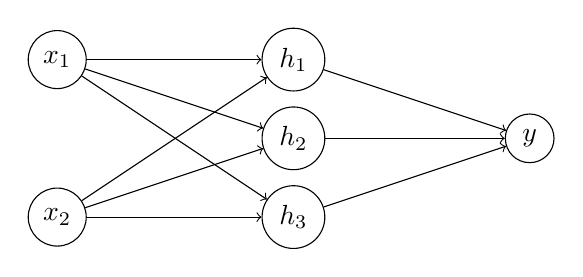
\begin{tikzpicture}
        \node[draw,circle] (x1) at (0,0) {$x_1$};
        \node[draw,circle] (x2) at (0,-2) {$x_2$};
        \node[draw,circle] (h1) at (3,0) {$h_1$};
        \node[draw,circle] (h2) at (3,-1) {$h_2$};
        \node[draw,circle] (h3) at (3,-2) {$h_3$};
        \node[draw,circle] (y) at (6,-1) {$y$};
        \draw[->] (x1) -- (h1);
        \draw[->] (x1) -- (h2);
        \draw[->] (x1) -- (h3);
        \draw[->] (x2) -- (h1);
        \draw[->] (x2) -- (h2);
        \draw[->] (x2) -- (h3);
        \draw[->] (h1) -- (y);
        \draw[->] (h2) -- (y);
        \draw[->] (h3) -- (y);
    \end{tikzpicture}
    \caption{Rete neurale di esempio}
    \label{fig:my_label}
\end{figure}

Ma passiamo alla definizione formale:

\textbf{Definizione Rete Neurale}: Una rete neurale è una tupla:
\begin{equation}
    NN = \{g,l,o,i,fpp\}
\end{equation}
con:
\begin{itemize}
    \item g: il grafico
    \item l: la funzione loss
    \item o: l'ottimizzatore
    \item i: l'inizializzatore
    \item fpp: la fix point procedure
\end{itemize}

\textbf{Nota 1:} l'ottimizzatore intende in quale modo si performa la \textbf{discesa del gradiente.}

\textbf{Nota 2:} l'inizializzatore è la funzione che inizializza i pesi della rete neurale. Ci possono essere diversi algoritmi per gli
inizializzatori, ma non c'è modo di sapere quale funziona meglio, poiché non si può sapere nelle reti neurali.

\subsubsection{Il grafo}

Il solito grafo che abbiamo visto in precedenza è un grafo aciclico diretto. Ha
dei nodi che sono i percettroni, che hanno degli archi composti dai pesi, che
hanno una funzione di attivazione, che prendono in input un valore e ne sputano
fuori uno chiamando la funzione di attivazione sull'input.

\textbf{Nota:} la funzione di attivazione è una funzione non lineare.

\subsubsection{La funnzione loss}

L'obiettivo della funzione loss è quello di misurare la distanza tra il valore
predetto e il valore reale.
\begin{equation}
    L(y,\hat{y}) = \frac{1}{2}(y-\hat{y})^2
\end{equation}

\subsubsection{L'ottimizzatore}

L'ottimizzatore ci permette di trovare una soluzione ottimale \textbf{non
    ottima}, cioé trovare \textbf{il minimo della funzione di loss}. La tecnica che
si usa è quella delle \textbf{discesa del gradiente}.

\subsubsection{Discesa del gradiente}

La discesa del gradiente sfrutta un parametro chiamato \textbf{learning rate}
che permette di capire quanto la discesa del gradiente deve essere veloce. Se
il learning rate è troppo alto, la discesa del gradiente potrebbe non
convergere, se è troppo basso, la discesa del gradiente potrebbe convergere
troppo lentamente.

\textbf{Nota:} il learning rate è un ottimizzatore \textit{molto naive}.

\subsubsection{Inizializzatore}

Il metodo di inizializzazione può cambiare di molto il risultato della rete
neurale. In pratica assegna un valore ai \textit{pesi} e ai \textit{bias}.
Alcuni metodi sono:
\begin{itemize}
    \item Inizializzazione a 0: Questo ha alcuni problemi, perché non si ha
          diversificazione tra i nodi e i nodi nascosti diventano simmetrici.
    \item inizializzazione costante: stessi problemi della precedente
    \item Inizializzazione Random: Si fa seguendo una distribuzione uniforme oppure una
          distribuzione normale.
\end{itemize}

\subsubsection{Fix Point Procedure}

La procedura per il training di una rete neurale è un processo che si basa su
alcuni steps:
\begin{lstlisting}

net CustomNeuralNetwork(...)
initialize_weights_and_biases (net)
optimizer = myOptimizer(...) 
loss_function = myLoss Function(...)
epochs = ... # the number of dataset scans
history = [] # a list containing the loss evolution
for epoch in range(epochs):
    optimizer.reset() # it may have an internal status
    loss = loss_fuction (out_target, net(input)) back_propagation (loss, optimizer, net)
    history.append(loss)
\end{lstlisting}

\subsection{Esempio da zero}
\subsubsection{La funzione Sigmoid}

Spendiamo qualche parola sulla funzione sigmoid, che è una funzione molto
importante per le reti neurali.

In particolare, la funzione avrà un valore di attivazione compreso tra 0 e 1 e,
in particolare, quando l'input è 0, la funzione ha valore 0.5. Se ha un valore
basso, sarà zero e chiaramente se sarà alto avrà valore 1.
\begin{figure}[H]
    \begin{center}
        \begin{tikzpicture}
            \begin{axis}[
                    axis lines = left,
                    xlabel = $x$,
                    ylabel = {$f(x)$},
                ]
                %Below the red parabola is defined
                \addplot [
                    domain=-10:10,
                    samples=100,
                    color=red,
                ]
                {1/(1+exp(-x))};
                \addlegendentry{$\frac{1}{1+e^{-x}}$}
            \end{axis}
        \end{tikzpicture}
    \end{center}
    \caption{Funzione Sigmoid}
\end{figure}

Detto questo, \textbf{per quale motivo è importante?} Se pensiamo
all'\textit{inizializzazione}, che tipi di valori è meglio avere? Avere tutti i
valori a zero porterebbe a valori simmetrici e quindi a problemi di
convergenza. Vogliamo dei valori di pesi che siano \textbf{distribuiti
    uniformemente intorno allo 0.}

\subsection{Tangente Iperbolica TanH}

La funzione TanH è una funzione che ha un valore di attivazione compreso tra -1
e 1 e, in particolare, quando l'input è 0, la funzione ha valore 0. Se ha un
valore basso, sarà -1 e chiaramente se sarà alto avrà valore 1.

\begin{figure}[H]
    \begin{center}
        \begin{tikzpicture}
            \begin{axis}[
                    axis lines = left,
                    xlabel = $x$,
                    ylabel = {$f(x)$},
                ]
                %Below the red parabola is defined
                \addplot [
                    domain=-10:10,
                    samples=100,
                    color=red,
                ]
                {tanh(x)};
                \addlegendentry{$tanh(x)$}
            \end{axis}
        \end{tikzpicture}
    \end{center}
    \caption{Funzione TanH}
\end{figure}

\subsection{ReLu}

La funzione ReLu è una funzione che ha un valore di attivazione pari a 0 quando
l'input è negativo e ha un valore di attivazione pari all'input quando l'input
è positivo.

\textbf{Parole di Adornetto:} E' buona? Si. E' stabile? Si. Perché? Boh.

\begin{figure}[H]
    \begin{center}
        \begin{tikzpicture}
            \begin{axis}[
                    axis lines = left,
                    xlabel = $x$,
                    ylabel = {$f(x)$},
                ]
                %Below the red parabola is defined
                \addplot [
                    domain=-10:10,
                    samples=100,
                    color=red,
                ]
                {max(0,x)};
                \addlegendentry{$max(0,x)$}
            \end{axis}
        \end{tikzpicture}
    \end{center}
    \caption{Funzione ReLu}
\end{figure}

\subsection{Scalare i valori}

Skip molto avanti riguardo l'esempio, ma si parla di scalare i dati.

Lo scaling dei dati è un'operazione importante nel machine learning perché i
dati possono essere su scale diverse e questo può causare problemi durante
l'allenamento del modello. Ad esempio, se abbiamo due variabili di input, una
che varia da 0 a 1 e l'altra che varia da 0 a 1000, la seconda variabile avrà
un impatto molto maggiore sull'output del modello rispetto alla prima. Ciò può
portare a problemi come l'overfitting, in cui il modello si adatta troppo ai
dati di addestramento e non generalizza bene sui dati di test.

Per risolvere questo problema, si utilizzano tecniche di scaling dei dati per
portare tutte le variabili su una scala comune. Ci sono diverse tecniche di
scaling, come la normalizzazione e la standardizzazione, che possono essere
utilizzate a seconda del tipo di dati e del modello utilizzato.

Le funzioni di attivazione, come la funzione ReLU, possono anche essere
influenzate dalla scala dei dati di input. Se i dati non sono scalati
correttamente, la funzione di attivazione potrebbe produrre valori che non
permettono un allenamento corretto del modello. Lo scopo dello scaling dei dati
è quello di mantenere i dati intorno allo 0, in modo che le funzioni di
attivazione possano produrre valori che permettono un allenamento corretto del
modello.

\begin{itemize}
    \item Standardizzazione: La standardizzazione è una tecnica di scaling dei dati che
          assume che i dati siano distribuiti normalmente all'interno di ogni feature e
          li scala in modo che la distribuzione abbia una media uguale a 0 e una
          deviazione standard uguale a 1. Questa tecnica funziona bene quando i dati
          hanno una distribuzione normale, ma non funziona bene se i dati hanno una
          distribuzione non normale.
    \item Normalizzazione: La normalizzazione è una tecnica di scaling dei dati che scala
          i valori di ogni feature in modo che siano compresi tra 0 e 1. Questa tecnica
          funziona bene quando i valori di input non hanno una distribuzione normale. Ad
          esempio, se i valori di input sono compresi tra 0 e 1000, la normalizzazione li
          porterà su una scala compresa tra 0 e 1.
\end{itemize}

\subsection{Plottare la loss}

La funzione loss è una misura dell'errore del modello durante
l'allenamento. L'obiettivo dell'allenamento è quello di minimizzare la funzione
loss, ovvero di ridurre l'errore del modello. Durante l'allenamento, il modello
viene eseguito su un set di dati di addestramento e la funzione loss viene
calcolata per ogni esempio di addestramento. L'errore totale del modello è la
somma di tutte le funzioni loss per ogni esempio di addestramento.

L'allenamento del modello avviene in epoche, ovvero in cicli di esecuzione su
tutti i dati di addestramento. L'obiettivo è che la funzione loss diminuisca ad
ogni epoca, ovvero che l'errore del modello diminuisca man mano che il modello
viene addestrato su più dati. Se la funzione loss non diminuisce ad ogni epoca,
significa che il modello non sta imparando abbastanza dai dati di addestramento
e potrebbe essere necessario modificare l'architettura del modello o i
parametri di addestramento.

Se la funzione di loss arriva a 0, vuol dire che \textbf{siamo in minimo globale}, che non è comune.

%make a plot with x = epochs and y = loss and loss reaches 0 at the end, with a curve that goes down
\begin{figure}[H]
    \begin{center}
        \begin{tikzpicture}
            \begin{axis}[
                    axis lines = left,
                    xlabel = $epochs$,
                    ylabel = {$loss$},
                ]
                %Below the red parabola is defined
                \addplot [
                    domain=0:10,
                    samples=100,
                    color=red,
                ]
                {1/(1+exp(x))};
                \addlegendentry{$loss$}
            \end{axis}
        \end{tikzpicture}
    \end{center}
    \caption{Funzione loss}
\end{figure}


Se invece finiami con un grafico che arriva fino a 0.1 e poi si stabilizza, 
potremmo essere in un \textbf{minimo locale}, oppure semplicemente la topologia della Rete
permette di avere questo risultato come massimo risultato.


\subsection{Importante cosa su Gradient Descent}

Lo usiamo per un motivo particolare:
\begin{quote}
    Più andiamo indietro nei layer della rete, maggiori saranno i termini 
    che abbiamo già calcolato, rendendo i calcoli più efficienti.
\end{quote}
Questo è più semplice rispetto ad invertire una matrice
\newpage

\end{document}